\documentclass[a4paper]{article}

\usepackage[english]{babel}
\usepackage[utf8x]{inputenc}
\usepackage{amsmath}
\usepackage{graphicx}
\usepackage[colorinlistoftodos]{todonotes}
\usepackage{schemabloc}
\usetikzlibrary{calc}

\newcommand{\mb}[1]{\mathbf{#1}}
\newcommand{\derivt}[1]{\frac{\mathrm{d}#1}{\mathrm{dt}}}
\newcommand{\deriv}[2]{\frac{\partial#1}{\partial#2}}

\title{AMORO Lab Part 2: Simulation of a five-bar mechanism}
\author{Damien SIX\\ damien.six@ls2n.fr}
\date{Released: August 20, 2021}

\begin{document}
\maketitle
\begin{figure}[h!]
\centering
\includegraphics[width=0.6\textwidth]{DexTAR_mp.jpg}
\caption{The DexTAR robot (Mecademic)}
\label{fig:DEXTAR}
\end{figure}
\section{Objective}
The main objective of the present lab is to compute the geometric, kinematic and dynamic models of a five-bar mechanism and to compare them with the results obtained with GAZEBO. Then, a controller will be designed to track a trajectory in simulation.

The kinematic architecture of the five-bar mechanism is shown in Fig.\ref{fig:5bar}. For the mechanism of the Gazebo mock-up, the geometric parameters are: 
\begin{itemize}
\item    Bar length (all bars are equal length): $l$ = 0.09 m 
\item    Distance between the two active joints: $d$ = 0.118 m 
\end{itemize}
and the base dynamic parameters are:
\begin{itemize}
    \item $ZZ_{1R}$ the grouped inertia on the first link of the left arm. \\$ZZ_{1R}$=0.002 kg.m²
    \item $ZZ_{2R}$, the grouped inertia on the first link of the right arm. \\$ZZ_{2R}$=0.002 kg.m²
    \item $m_R$ the grouped mass on the end-effector. $m_R=0.5$ kg
\end{itemize}
    
\begin{figure}[h!]
\centering
\includegraphics[width=0.6\textwidth]{RuRRRRu_kin.eps}
\caption{Kinematic architecture of the five-bar mechanism. Joints located at A11 and A21 are actuated.}
\label{fig:5bar}
\end{figure}


\section{Help for the LAB} 
Some computations required for this lab are given in the course and recalled in the appendix \textit{Computation of the five-bar mechanism models}. This help is provided for the Five-Bar. For the Biglide mechanism (Part~3 of the Lab), a similar document is a \textbf{deliverable} from the lab. To avoid, loosing time for Part~3, it is \textbf{mandatory} to prepare this document \textbf{BEFORE} getting to Part~3 during the lab. As a consequence, this should be done \textbf{AT HOME} and not during the lab sessions.

\section{Kinematic models of the five-bar mechanism}
\label{analysis}
In the first part of this lab, we will simulate the kinematic behavior of the five-bar mechanism and compare it with GAZEBO output. To run the lab, execute the following steps:
\begin{enumerate}
    \item Run Gazebo using the command \textit{ros2 launch lab\_amoro gazebo.launch.py}
    \item Insert the appropriate model by selecting the \textit{insert} tab then the \textit{FiveBar} model.
\end{enumerate}
You can now go in the \textit{student\_scripts} folder and complete the models in the file \textit{five\_bar\_models.py}. You should not modify the input-output of the functions but just put the appropriate computation. To check that the models are properly computed, you must run the \textit{model\_test.py} script for the direct models and \textit{inverse\_model\_test.py} for the inverse ones. To run the python scripts, just go in the \textit{student\_scripts} using the terminal and use the command\\
\$ python3 your\_script.py
\\
%
All the following models must be validated
\begin{itemize}
    \item The Direct Geometric Model
    \item The Direct Geometric Model for passive joints
    \item The Inverse Geometric Model
    \item The First Order Kinematic Model
    \item The First Order Kinematic Model for passive joints
    \item The Inverse First Order Kinematic Model
    \item The Second Order Kinematic Model
    \item The Second Order Kinematic Model for passive joints
    \item The Inverse Second Order Kinematic Model
\end{itemize}
%
\textbf{Python math and numpy libraries:}\\
To code the computation of your models. It is recommended to use the \textit{math} and \textit{numpy} libraries. \textit{math} will contain the trigonometric functions you need and \textit{numpy} allows the manipulation of arrays and matrices. \textit{numpy} is usually imported under the alias \textit{np}. The following methods will be handy.
\begin{itemize}
    \item v = np.array([0.0, 1.0]) to create a 2D vector $\mathbf{v}$
    \item M = np.array([[0.0, 1.0], [2.0, 3.0]]) to create a 2D matrix $\mathbf{M}$
    \item u.dot(v) for the dot product of two vectors
    \item M.dot(v) for the multiplication for the product $\mathbf{M}\mathbf{v}$
    \item np.matmul(M, N) for the matrix multiplication $\mathbf{M}\mathbf{N}$
    \item np.linalg.inv(M) for the matrix inversion
    \item M.transpose() for the matrix transpose
\end{itemize}
%
\section{Computed torque control}
%
\subsection{Trajectory generation}
%
\textbf{Recall:} A polynomial trajectory is defined with initials conditions and final conditions (eventually intermediate). The number of initial and final conditions will determine the order of the polynomial used for the trajectory (number of conditions -1). 

As an example, displacement in $x$ with initial and final positions and velocities (4 conditions) requires a 3$^{\text{rd}}$ order polynomial function.
%
\begin{equation}
x=a_1t^3+a_2t^2+a_3t+a_4\nonumber
\end{equation}
%
The initials and final conditions are expressed as
\begin{align*}
x(t_i)&=a_1t_i^3+a_2t_i^2+a_3t_i+a_4\\
\dot{x}(t_i)&=3a_1t_i^2+2a_2t_i+a_3\\
x(t_f)&=a_1t_f^3+a_2t_f^2+a_3t_f+a_4\\
\dot{x}(t_f)&=3a_1t_f^2+2a_2t_f+a_3
\end{align*}
which can be put in the form of a linear system
%
\begin{equation}
\mathbf{P}\mathbf{a}=\mathbf{c}\nonumber
\end{equation}
%
with $\mathbf{a}=(a_1,a_2,a_3,a_4)^T$ containing the coefficients of the polynomial function. Solving this linear system gives the polynomial coefficients for the trajectory.

A trajectory between two points \textit{A}($x_A, y_A$) and B($x_B, y_B$), with null velocity and acceleration at initial and final position, in the time interval [0, $t_f$] is given by a fifth order polynomial function. This specific case can be expressed as: 
\begin{align*}
x(t)&=x_A+s(t)(x_B-x_A)\\
y(t)&=y_A+s(t)(y_B-y_A)
\end{align*}
with
\begin{equation*}
s(t)=10\left(\frac{t}{t_f}\right)^3-15\left(\frac{t}{t_f}\right)^4+6\left(\frac{t}{t_f}\right)^5
\end{equation*}
%

\textbf{To do:} In the \textit{control.py} file, write down a function to compute the trajectory in Cartesian space as a numpy array given some initial position, final position and duration. The function should output position, velocity and acceleration for each coordinate. The trajectory should be sampled with a 10 ms sampling time.

Write down a second function to compute the trajectory (position, velocity, acceleration) in joint space from Cartesian space using the inverse geometric and kinematic models.
%
\subsection{Introduction to Computed Torque Control}
%
The Computed Torque Control is based on the feedback linearization of the system through the inverse dynamic model. The dynamic model of a parallel robot can be written under the generic form 
	%
	\begin{equation*}
	\boldsymbol{\tau}=\mathbf{M}\ddot{\mathbf{q}}_a+\mathbf{c} \nonumber
	\end{equation*}
	%
	$\mb{M}$ being the inertia matrix, definite positive and $\mathbf{c}$ the vectore of Coriolisis and Centrifugal effects.
	%
	Considering the input $\boldsymbol{\tau}$ this system in non-linear, an auxiliary control input is defined  $\boldsymbol{\alpha}$
	%
	\begin{equation*}
	\boldsymbol{\alpha}=\mathbf{M}^{-1}(\boldsymbol{\tau}-\mathbf{c})
	\end{equation*}
	%
    If the dynamic model is accurate, this auxiliary input correspond to the robot acceleration.
	%
	\begin{equation*}
	\boldsymbol{\alpha}=\ddot{\mathbf{q}}_a
	\end{equation*}
    %
    A PD control law can be applied on this auxiliary input
	%
	\begin{equation*}
	\boldsymbol{\alpha}=\ddot{\mathbf{q}}_{t}+\mathbf{K}_d(\dot{\mathbf{q}}_{t}-\dot{\mathbf{q}}_a)+\mathbf{K}_p(\mathbf{q}_{t}-\mathbf{q}_a)
	\end{equation*}
    %
    With $\mathbf{K}_p$ et $\mathbf{K}_d$ definite positive (usually positive diagonal matrices). 
	The torque input is deduced from this auxiliary control law\textcolor{red}{
	\begin{align*}
\boldsymbol{\tau}&=\mathbf{M}\boldsymbol{\alpha}+\mathbf{c}\\
    &=\mathbf{M}(\ddot{\mathbf{q}}_{t}+\mathbf{K}_d(\dot{\mathbf{q}}_{t}-\dot{\mathbf{q}}_a)+\mathbf{K}_p(\mathbf{q}_{t}-\mathbf{q}_a))+\mathbf{c}	
	\end{align*}}

	%
	Fig.\ref{fig:CTC} shows the controller scheme. 	With $\mathbf{\tilde{\mb{q}}}=\mathbf{q}_{ref}-\mathbf{q}_a$, the closed-loop equation of the control system is 
	%
	\begin{figure}
		\centering
		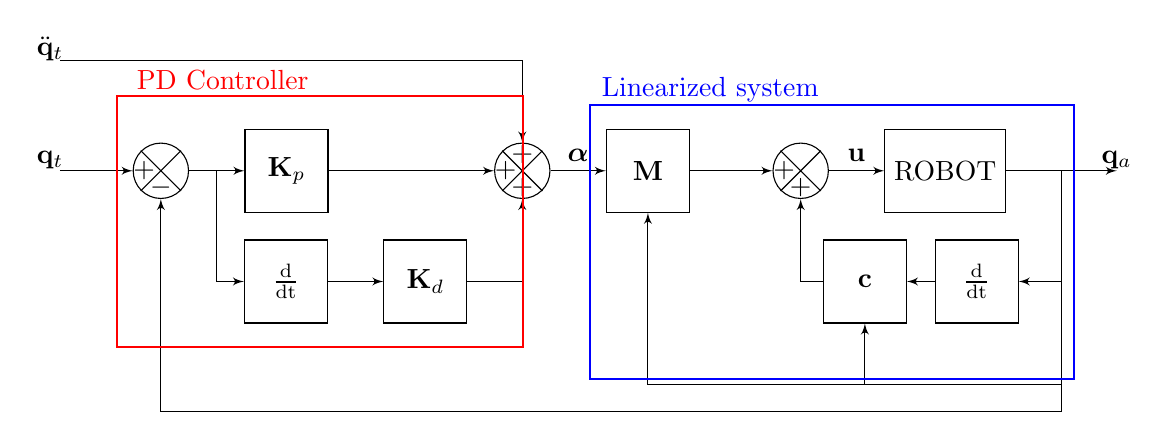
\begin{tikzpicture}
		%Entrée
		\sbEntree{q}
		\sbDecaleNoeudy[-4]{q}{qdd}
		\sbDecaleNoeudy[4]{q}{int}
		\sbNomLien{q}{$\mathbf{q}_{t}$}
		\sbNomLien{qdd}{$\ddot{\mathbf{q}}_{t}$}
		\sbComp{comp}{q}
		\sbRelier{q}{comp}	
		
		\sbBloc{Kp}{$\mathbf{K}_p$}{comp}
		\sbRelier{comp}{Kp}
		\sbCompSum[7]{sum}{Kp}{+}{+}{+}{}
		\sbRelier{Kp}{sum}
		\sbDecaleNoeudy[4]{comp}{deriv}
		\sbBloc[3]{d3}{$\derivt{}$}{deriv}
		\sbBlocL{kd}{$\mathbf{K}_d$}{d3}
		\sbRelierxy{kd}{sum}
		\sbRelierxy{qdd}{sum}
		\sbRelieryx{comp-Kp}{d3}
		%Innerloop
		\sbBloc{M}{$\mathbf{M}$}{sum}
		\sbRelier[$\boldsymbol{\alpha}$]{sum}{M}
		\sbCompSum{sum2}{M}{}{+}{+}{}
		\sbRelier{M}{sum2}
		\sbBloc{robot}{ROBOT}{sum2}
		\sbRelier[$\mb{u}$]{sum2}{robot}
		\sbDecaleNoeudy[4]{sum2}{inloop}
		\sbBloc[0.8]{H}{$\mathbf{c}$}{inloop}
		\sbBloc[1]{d4}{$\derivt{}$}{H}
		\sbSortie[4]{s}{robot}
		\sbRelier{robot}{s}
		\sbNomLien{s}{$\mathbf{q}_a$}
		\sbRelieryx{robot-s}{d4}
		\sbRelier{d4}{H}
		\sbRelierxy{H}{sum2}
		%Renvois
		\sbRenvoi[7]{robot-s}{H}{}
		\sbRenvoi[7]{robot-s}{M}{}
		\sbRenvoi[8]{robot-s}{comp}{}
		%Groupes
		\draw[red,thick] ($(comp.north west)+(-0.3,0.7)$) rectangle ($(kd.south east)+(0.7,-0.3)$);
		\node at ($(comp.north west)+(-0.3,0.9)$) [label=right:\textcolor{red}{PD Controller}]{};
		\draw[blue,thick] ($(M.north west)+(-0.2,0.3)$) rectangle ($(d4.south east)+(0.7,-0.7)$);
		\node at ($(M.north west)+(-0.3,0.5)$) [label=right:\textcolor{blue}{Linearized system}]{};
		\end{tikzpicture}
		\caption{Computed Torque Control Scheme}
		\label{fig:CTC}
	\end{figure}
	%

	%
	\begin{equation*}
	\ddot{\tilde{\mb{q}}}+\mathbf{K}_d\dot{\tilde{\mb{q}}}+\mathbf{K}_p\tilde{\mb{q}}=\mb{0}
	\end{equation*}
	%
	Ensuring the convergence of the error $\tilde{\mb{q}}$ toward $\mathbf{0}$. 
%
\subsection{Computed Torque Control simulation}
\begin{itemize}
    \item Using the Robot class input and output, code in \textit{control.py} a computed torque control to track a desired trajectory.
    \item Define a trajectory between the initial position (0.09,0.06796322) and the position (0,0.1) in 2s.
    \item Run the simulation and check the trajectory tracking performed.
    \item Define a trajectory between the initial position (0.09,0.06796322) and the position (0.05, 0.0) in 4.0s. What happens? Explain why (hint, plot the joint effort you ask)
\end{itemize}
%
\end{document}
  




